\chapter{Transverse Asymmetry}
The Beam Normal Single Spin Asymmetry (BNSSA, also known as Transverse Single Spin Asymmetry
or Transverse Asymmetry) is different from the PV asymmetry, it is purely 
electromagnetic and therefore parity-conserving. It arises from the interference
between one-photon and two-photon exchange (OPE and TPE), therefore it is sensitive 
to the TPE amplitude. By measuring it, we can probe the strength of TPE, an 
important knowledge of electron elastic scattering that may explain the myth
of proton radius measured with different methods.

The transverse asymmetry is also an important systematic uncertainty to our PV 
asymmetry measurement, because there is always some residual transverse polarization
in the electron beam. With $\CA_n \sim \alpha_{EM}m_e/E_e$, its magnitude of $10^{-5}$
for a GeV level electron beam is much larger than $\CA_{pv}$, so a complete 
understanding and precise measurement of the transverse asymmetry is needed
to ensure accurate correction of $\CA_{pv}$.

Being a routine and bonus of a PV experiment, PREX-I also measured the transverse
asymmetry of some nuclei, namely ${}^{1}H$, \He, \C and \Pb. Surprisingly, PREX-I
saw a zero transverse asymmetry in \Pb, while the transverse asymmetries of other 
light nuclei seemed to agree with theoretical predictions, as shown in 
Fig.~\ref{fig:PREX-I_AT}. One of the reason for PREX-II was that we wanted to
verify the zero measurement in \Pb, which remains as a challenge to theorists.
\begin{figure}
    \centering
    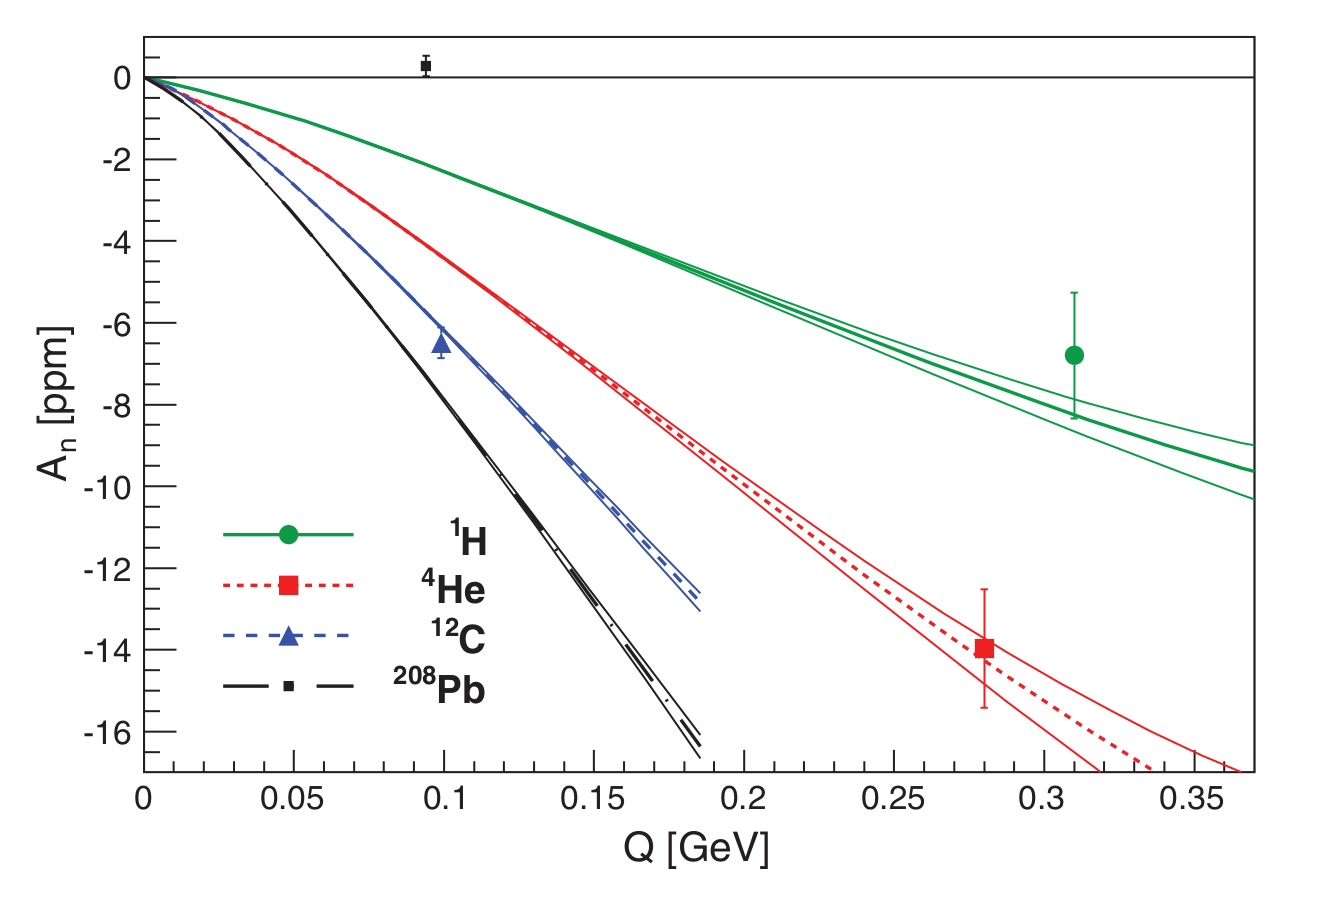
\includegraphics[width=0.5\linewidth]{PREX-I_AT}
    \caption{Transverse asymmetry measured in PREX-I.}
    \label{fig:PREX-I_AT}
\end{figure}

As its name implies, BNSSA depends on only one spin, either the target or the
electron, polarized target is better that polarized target in that it is hard
to polarize nuclei, especially heavy nuclei.

%%%%%%%%%%%%%%%%%%%%%%%%%%%%%%%%%%%%%%%%%%%%%%%%%%%%%%%%%%%%%%%%%%%%%%%%
\section{Motivation for Transverse Asymmetry}

%%%%%%%%%%%%%%%%%%%%%%%%
\subsubsection{The Scattering Theory}
Consider the scattering of a free ($t_0 \rightarrow -\infty$) particle from a 
time independent potential $V(\vec{r})$, 
which decays quickly as $r \rightarrow \infty$. The evolution from the free initial state
$\ket{i}$ is denoted as $\ket{\psi(t)}_S$ (under the Schr\"odinger picture, $\hbar = 1$):
\begin{equation}
    \ket{\psi(t)}_S = U(t)\ket{\psi(t_0)} = \lim_{t_0 \rightarrow -\infty}U(t, t_0)\ket{i}
\end{equation}
where $U(t, t_0)$ is the evolution operator:
\begin{equation}
    U(t, t_0) = \exp(\frac{1}{i}(H_0 + V)(t - t_0)) = \exp(-i(H_0 + V)(t-t_0))
\end{equation}
$H_0$ is the free Hamiltonian and $H = H_0 + V$ is the complete Hamiltonian
with interaction term. 

The projection of $\psi(t)$ to a free final state $\ket{f}$ defines the so called
S-matrix (the order of the subscripts matters):
\begin{equation}
    S_{if} \equiv \lim_{t\rightarrow +\infty}\bra{f}\ket{\psi(t)} 
    = \lim_{t\rightarrow\infty} \lim_{t_0 \rightarrow -\infty} \bra{f} U(t, t_0) \ket{i}
\end{equation}
Which defines the S operator:
\begin{equation}
    S_{if} = \bra{f} S \ket{i} \Longrightarrow S = U(+\infty, -\infty)
\end{equation}

The S-matrix describe the scattering amplitude from the free initial state $\ket{i}$
to the free final state $\ket{f}$. Conservation of probability indicates
unitary of S matrix:
\begin{equation}
    S^\dag S = \sum_f |\bra{f} U(+\infty, -\infty) \ket{i}|^2 = 1
\end{equation}

It is easier to evaluate $U(t)$ in the interaction picture. Define
\begin{equation}
    \ket{\psi(t)}_I \equiv \exp(-\frac{1}{i}H_0 t) \ket{\psi(t)}_S 
    = \exp(iH_0 t) \exp(-i (H_0 + V) t)\ket{i}
\end{equation}
The subscript I and S denote the interaction and Schr\"odinger picture respectively.
The evolution of $\ket{\psi(t)}_I$ is:
\begin{equation}
    \begin{aligned}
	\frac{d}{dt}\ket{\psi(t)}_I 
	&= \left[ \exp(i H_0 t) (iH_0) \exp(-i (H_0 + V) t)
	+ \exp(i H_0 t) (-i)(H_0 + V) \exp(-i (H_0 + V) t) \right] \ \ket{i}  \\
	&= -i\ \exp(i H_0 t)\ V \ \exp(-i (H_0 + V) t) \ket{i}   \\
	&= -i \exp(iH_0 t) V \exp(-iH_0 t) \cdot \exp(iH_0 t) \exp(-i(H_0 + V)t) \ket{i}   \\
	&= -i V_I(t) \ket{\psi(t)}_I
    \end{aligned}
    \label{eq:interaction_evolution}
\end{equation}
where $V_I(t) = \exp(iH_0t)V\exp(-iH_0t)$ is the time dependent interaction term.
Eq.~\ref{eq:interaction_evolution} leads to the Dyson series:
\begin{equation}
    U(t, t_0) = 1 - i\int_{t_0}^t dt_1 V_I(t_1) U(t_1, t_0) = \sum_{n=0}^\infty \frac{(-i)^n}{n!}\int_{t_0}^t dt_1 \cdots \int_{t_0}^t dt_n T[V_I(t_1)\cdots V_I(t_n)]
\end{equation}
T means time-ordering:
\begin{equation}
    T(V_I(t_1) V_I(t_2)) \equiv 
    \begin{cases}
	V_I(t_1)V_I(t_2)    & t_1 \le t_2   \\
	V_I(t_2)V_I(t_1)    & t_2 \le t_1   \\
    \end{cases}
\end{equation}

\begin{equation}
    \begin{aligned}
	\bra{f} U(t, t_0) \ket{i} 
	&= \bra{f}\ket{i} - i \bra{f} \int_{t_0}^t dt_1 V_I(t_1) U(t_1, t_0) \ket{i}	\\
	&= \delta_{if} - i\sum_m \int_{t_0}^t dt_1 \bra{f}\exp(iH_0 t_1) V \exp(-iH_0 t_1)(t_1)\ket{m} \bra{m} U(t_1, t_0) \ket{i} \\
	&= \delta_{if} - i\sum_m \bra{f}V\ket{m} \int_{t_0}^t dt_1 \exp(i(E_f - E_m)t_1) \bra{m}U(t_1, t_0)\ket{i}  \\
    \end{aligned}
    \label{eq:finite_S-matrix}
\end{equation}
Truncate Eq.~\ref{eq:finite_S-matrix} into first order ($\bra{m} U(t_1, t_0) \ket{i} = \delta_{im}$)
and define $T_{if} = \bra{f} V \ket{i}$, we will get:
\begin{equation}
    \bra{f} U(t, t_0) \ket{i} = \delta_{if} - iT_{if} \int_{t_0}^t dt_1 \exp(i(E_f - E_i)t_1)
\end{equation}
and 
\begin{equation}
    \begin{aligned}
	S_{if} &= \lim_{t\rightarrow +\infty}\lim_{t_0 \rightarrow -\infty} \bra{f} U(t, t_0) \ket{i}    \\
	    &= \delta_{if} - iT_{if} \int_{-\infty}^{\infty} dt_1 \exp(i(E_f - E_i)t_1)	\\
	    &= \delta_{if} + i2\pi\delta(E_f - E_i)T_{if}   \\
    \end{aligned}
\end{equation}
In matrix form:
\begin{equation}
    S = 1 + i2\pi T
\end{equation}
S begin unitary implies
\begin{equation}
    S^\dag S = (1 - i2\pi T^\dag) (1 + i2\pi T) = 1 + i2\pi(T - T^\dag) + (2\pi)^2 T^\dag T = 1
\end{equation}
which reads
\begin{equation}
    T - T^\dag = i (2\pi)T^\dag T = i(2\pi) T T^\dag
\end{equation}
In terms of matrix element:
\begin{equation}
    \begin{gathered}
    \delta(E_f - E_i)(T_{if} - T^\dag_{if}) = \sum_m i2\pi\delta(E_f - E_m)\delta(E_m - E_i)T_{fm}T^\dag_{mi}	\\
    T_{if} - T^\dag_{if} = \sum_m i2\pi\delta(E_m - E_i)T_{fm}T^\dag_{mi} = ia_{if} \\
    \end{gathered}
\end{equation}
where 
\begin{equation}
    a_{if} = \sum_m (2\pi) \delta(E_m - E_i)T_{fm}T^\dag_{mi}
\end{equation}
is the absorptive part of the transition amplitude $T_{if}$. $\ket{m}$ extends
to all on-shell intermediate states.

The two parts of S are easy to understand.
The constant piece denotes the evolution of one free particle into another free
particle without any interactions; obviously, it can evolve only into itself.
The T matrix describe the interaction (transition amplitude) between the free
initial particle $\ket{i}$ and the free final particle $\ket{j}$, which tells
us the interaction cross section.

The free particle state can be completely described by its momentum (ignoring spin
for now) $\vec{p}$. For an incoming electron $\ket{\vec{p}_i}$, the probability
to transform into the final state of $\ket{\vec{p}_f}$ is:
\begin{equation}
    dP = (phase\ space) \times (transition\ probability) = \frac{d\vec{p}_f}{(2\pi)^3} \times |S_{\vec{p}_i\vec{p}_f}|^2
\end{equation}
For a non trivial case of $\ket{f} \ne \ket{i}$, we have:
\begin{equation}
    S_{if} = i2\pi \delta(E_f - E_i)T_{if}
\end{equation}
The differential cross section will be:
\begin{equation}
    d\sigma = \frac{dP}{\CL \Delta t}
\end{equation}
where $\CL$ is the luminosity, indicating number of particles hitting 
the target per unit area per unit time, in our case of incoming plane wave, 
$\CL = \rho v = v$, and $\Delta t$ is the interaction time.
\begin{equation}
    d\sigma = \frac{1}{v\Delta t} \frac{d\vec{p}_f}{(2\pi)^3} 2\pi\delta(E_f - E_i) \left. 2\pi\delta(E_f - E_i)\right|_{E_f = E_i} |T_{if}|^2
\end{equation}
Transform one $\delta$ back to integrating form: 
\begin{equation}
    \left. 2\pi\delta(E_f - E_i) \right|_{E_f = E_i} 
    = \int_{-\infty}^{+\infty} dt \left.\exp(-i(E_f - E_i)t)\right|_{E_f = E_i}
    = \int_{-\infty}^{+\infty} dt 
\end{equation}
Physically, we don't go back or into infinity in time, because the real particle
is a finite wave packet rather than a plane wave. The integration above should 
be finite and close to the interaction time
\begin{equation}
    \int_{-\infty}^{+\infty} dt \rightarrow \Delta t
\end{equation}
Thus we have a defined cross section
\begin{equation}
    d\sigma = \frac{1}{v} \frac{d\vec{p}_f}{(2\pi)^3} 2\pi\delta(E_f - E_i) |T_{if}|^2
\end{equation}
The cross section is proportional to $|T_{if}|^2$, as known to us.


%%%%%%%%%%%%%%%%%%%%%%%%
\subsubsection{T-Symmetry}
Symmetry is the most profound concept and foundation of modern physics, which
can be separated into continuous symmetries and discrete ones. Time symmetry
is one important discrete symmetry, which states that physical laws should
keep unchanged under time reversal operation. Time reversal is the operation
that flips time arrow, so that time runs backward after time reversal. Obviously, 
vectors that are first order of time derivative will also reverse sign, such
as momentum, angular momentum and magnetic field.

Express the time reversal operation in QM:
\begin{equation}
    \ket{\tilde{\psi}} = \hat{\mathcal{T}} \ket{\psi} 
\end{equation}
where $\hat{\mathcal{T}}: t \rightarrow -t$ is the time reversal operator. 

In terms of our scattering, as said above, a particle will flip its momentum 
and spin (angular momentum) under time reversal, and pick up a phase.
\begin{equation}
    \ket{\tilde{\psi}} = \hat{\mathcal{T}} \ket{\psi_\uparrow(\vec{k})} = \eta\ket{\psi_\downarrow(-\vec{k})}
\end{equation}
$\eta$ is the phase difference, $|\eta|^2 = 1$. So the T matrix can also be applied
to time reversed state
\begin{equation}
    T_{\tilde{i}\tilde{f}} = \bra{\tilde{f}} V \ket{\tilde{i}}
\end{equation}

It is well known that electromagnetic interaction is invariant under time reversal.
\begin{equation}
    |T_{if}|^2 = |T_{\tilde{f}\tilde{i}}|^2 
\end{equation}

With these concepts, one can also define the \textbf{T-odd} quantities which
are proportional to the difference of the magnitude of a normal T element and 
its half time reversed version:
\begin{equation}
    \begin{aligned}
	\text{T-odd} &\propto |T_{if}|^2 - |T_{\tilde{i}\tilde{f}}|^2	\\
	    &= |T_{if}|^2 - |T_{fi}|^2	\\
	    &= |T_{if}|^2 - |T^\dag_{if}|^2	\\
	    &= |T_{if}|^2 - |T_{if} - ia_{if}|^2	\\
	    &= -i(T_{if}a^*_{if} - T^*_{if}a_{if}) - |a_{if}|^2	\\
	    &= 2Im(T_{if}a^*_{if}) - |a_{if}|^2
    \end{aligned}
    \label{eq:T-odd}
\end{equation}

%%%%%%%%%%%%%%%%%%%%%%%%
\subsubsection{Transverse Asymmetry}
Denote the incoming and outgoing transversely polarized electrons as 
$\ket{\vec{k}}$ and $\ket{\vec{k}'}$, the scattering is shown in Fig.~\ref{fig:transverse_scattering}.
\begin{figure}[h!]
    \centering
    \begin{subfigure}[c]{0.4\linewidth}
	\begin{tikzpicture}[scale=0.8]
	    \begin{feynman}[transform shape]
		\vertex (i1) {$e^-$};
		\vertex [right=1.0cm of i1, inner sep=0pt] (spin) {$\odot$};
		\vertex [right=2.3cm of spin] (ip);
		\vertex [right=2.8cm of ip] (i2) {A};
		\vertex [above right = 2cm and 2cm of ip] (o1) {$e^-$};
		\vertex [below left = 2cm and 2cm of ip] (o2) {A};

		\diagram* { {[edge=fermion]
		    (spin) --[edge label=$\vec{k}$] (ip) [dot] --[edge label = $\vec{k}'$] (o1),
		    (i2) --[edge label=$\vec{p}$](ip) [dot] -- [edge label = $\vec{p}'$]  (o2)},
		    (i1) -- (spin)
		};
	    \end{feynman}
	\end{tikzpicture}
    \end{subfigure}
    \hspace{0.2 cm}
    \textbf{-}
    \hspace{0.5 cm}
    \begin{subfigure}[c]{0.4\linewidth}
	\begin{tikzpicture}[scale=0.8]
	    \begin{feynman}[transform shape]
		\vertex (i1) {$e^-$};
		\vertex [right=1.0cm of i1, inner sep=0pt] (spin) {$\otimes$};
		\vertex [right=2.3cm of spin] (ip);
		\vertex [right=2.8cm of ip] (i2) {A};
		\vertex [above right = 2cm and 2cm of ip] (o1) {$e^-$};
		\vertex [below left = 2cm and 2cm of ip] (o2) {A};

		\diagram* { {[edge=fermion]
		    (spin) --[edge label=$\vec{k}$] (ip) [dot] --[edge label = $\vec{k}'$] (o1),
		    (i2) --[edge label=$\vec{p}$](ip) [dot] -- [edge label = $\vec{p}'$]  (o2)},
		    (i1) -- (spin)
		};
	    \end{feynman}
	\end{tikzpicture}
    \end{subfigure}
    \caption{Feynman plots of transversely polarized electron scatters off
    unpolarized nuclear target in the CoM. } 
    \label{fig:transverse_scattering}
\end{figure}

The transverse asymmetry will be:
\begin{equation}
    \CA_n \equiv \frac{N_{\uparrow} - N_{\downarrow}}{N_{\uparrow} + N_{\downarrow}} 
    = \frac{|T_{\uparrow}(\vec{k}, \vec{k}')|^2 - |T_{\downarrow}(\vec{k}, \vec{k}')|^2}{|T_{\uparrow}(\vec{k}, \vec{k}')|^2 + |T_{\downarrow}(\vec{k}, \vec{k}')|^2}
\end{equation}
where $T(\vec{k}, \vec{k}') = \bra{\vec{k}'} V \ket{\vec{k}}$ is the scattering
amplitude and the arrow subscript indicates electron's spin direction.
$T_\downarrow(\vec{k}, \vec{k}')$ is related to $T_\downarrow(-\vec{k}, -\vec{k}')$
by a rotation around the normal direction of the scattering plane, as shown in
Fig.~\ref{fig:rotation_plot}
\begin{figure}[h!]
    \centering
    \begin{subfigure}[c]{0.4\linewidth}
	\begin{tikzpicture}[scale=0.8]
	    \begin{feynman}[transform shape]
		\vertex (i1) {$e^-$};
		\vertex [right=1.0cm of i1, inner sep=0pt] (spin) {$\odot$};
		\vertex [right=2.3cm of spin] (ip);
		\vertex [right=2.8cm of ip] (i2) {A};
		\vertex [above right = 2cm and 2cm of ip] (o1) {$e^-$};
		\vertex [below left = 2cm and 2cm of ip] (o2) {A};

		\diagram* { {[edge=fermion]
		    (spin) --[edge label=$\vec{k}$] (ip) [dot] --[edge label = $\vec{k}'$] (o1),
		    (i2) --[edge label=$\vec{p}$](ip) [dot] -- [edge label = $\vec{p}'$]  (o2)},
		    (i1) -- (spin)
		};
	    \end{feynman}
	\end{tikzpicture}
    \end{subfigure}
    \hspace{0.2 cm}
    $\Longrightarrow$
    \hspace{0.5 cm}
    \begin{subfigure}[c]{0.4\linewidth}
	\begin{tikzpicture}[scale=0.8]
	    \begin{feynman}[transform shape]
		\vertex (i1) {$e^-$};
		\vertex [left=1.0cm of i1, inner sep=0pt] (spin) {$\odot$};
		\vertex [left=2.3cm of spin] (ip);
		\vertex [left=2.8cm of ip] (i2) {A};
		\vertex [below left = 2cm and 2cm of ip] (o1) {$e^-$};
		\vertex [above right = 2cm and 2cm of ip] (o2) {A};

		\diagram* { {[edge=fermion]
		    (spin) --[edge label=$\vec{k}$] (ip) [dot] --[edge label = $\vec{k}'$] (o1),
		    (i2) --[edge label=$\vec{p}$] (ip) [dot] -- [edge label = $\vec{p}'$] (o2)},
		    (i1) -- (spin)
		};
	    \end{feynman}
	\end{tikzpicture}
    \end{subfigure}
    \caption{Rotation by $\pi$ around the normal direction.} 
    \label{fig:rotation_plot}
\end{figure}
\begin{equation}
    T_\downarrow(\vec{k}, \vec{k}') = e^{i\pi} T_\downarrow(-\vec{k}, -\vec{k}')
\end{equation}

Let $T_{if} = T_{\uparrow}(\vec{k}, \vec{k}')$, then $T_{\tilde{i}\tilde{f}} = T_\downarrow (-\vec{k}, -\vec{k}')$
and
\begin{equation}
    \begin{aligned}
	\CA_n &\approx \frac{|T_{\uparrow}(\vec{k}, \vec{k}')|^2 - |T_{\downarrow}(-\vec{k}, -\vec{k}')|^2}{2|T_{\uparrow}(\vec{k}, \vec{k}')|^2} \\
	    &= \frac{|T_{if}|^2 - |T_{\tilde{i}\tilde{f}}|^2}{2|T_{if}|^2}  \\
	    &= \frac{2Im(T_{if}a^*_{if}) - |a_{if}|^2}{2|T_{if}|^2}
    \end{aligned}
    \label{eq:transverse_asymmetry}
\end{equation}

We see that the transverse asymmetry is a T-odd quantity. For EM interaction
\begin{equation}
    T_{if} \propto \alpha \qquad a_{if} \propto \alpha^2
\end{equation}
Because $\alpha \simeq \frac{1}{137}$ is small, we can expand Eq.~\ref{eq:transverse_asymmetry} 
in order of $\alpha$. To the lowest order
\begin{equation}
    \CA_n = 0
    \label{eq:AT_0}
\end{equation}
and to the first order 
\begin{equation}
    \CA_n = \frac{Im(T_{if}a^*_{if})}{|T_{if}|^2}
    \label{eq:AT_1}
\end{equation}

$T_{ij}$ represents the OPE interaction while $a_{ij}$ represents
the TPE interaction. So the physical interpretation of
Eq.~\ref{eq:AT_0} and \ref{eq:AT_1} is that time reversal symmetry requires 
the transverse asymmetry to be zero under the Born approximation (OPE only)
and the (lowest order) non-zero transverse asymmetry comes from the interference 
between OPE and TPE.
\begin{figure}[h!]
    \centering
    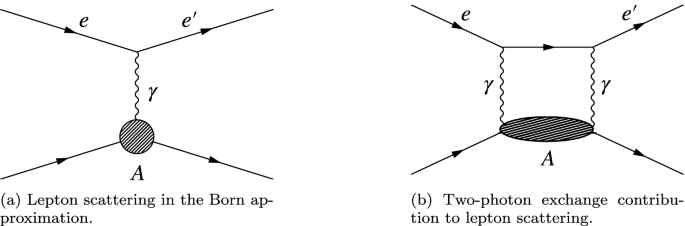
\includegraphics[width=0.8\linewidth]{at/OPE_n_TPE}
\end{figure}

%%%%%%%%%%%%%%%%%%%%%%%%%%%%%%%%%%%%%%%%%%%%%%%%%%%%%%%%%%%%%%%%%%%%%%%%
\section{How to Measure the Transverse Asymmetry: the Method}
The experimentally measured transverse asymmetry will be
\begin{equation}
    \CA_{mea} = \CA_n \vec{p}_e \cdot \hat{n} = \CA_n P_n \sin(\phi_s - \phi_e) = \CA_n P_n \sin\phi
    \label{eq:measured_AT}
\end{equation}
where $\vec{p}_e$ is the electron spin vector, whose magnitude is the polarization,
and $\phi_s$ being its angle w.r.t. the lab horizontal plane; 
$\hat{n} = \frac{\vec{k} \times \vec{k}'}{|\vec{k} \times \vec{k}'|}$ 
is the unit normal vector of the scattering plane and $\phi_e$ the angle between
the scattering plane and the lab horizontal plane. As shown in Fig.~\ref{fig:AT_scattering}.
So $\phi = \phi_s - \phi_e$ is angle between the spin vector and the scattering plane.
\begin{figure}[h!]
    \centering
    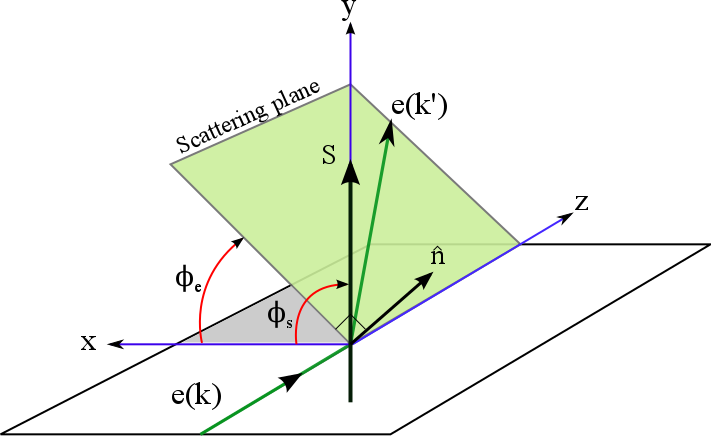
\includegraphics[width=0.7\linewidth]{AT_scattering}
    \caption{Schematic plot of scattering of transversely polarized electron.}
    \label{fig:AT_scattering}
\end{figure}

We see an angle dependence of the measured transverse asymmetry. Experimentally,
it is convenient to select the angle $\phi$ being $90^\circ$, which
usually set the lab horizontal plane as the scattering plane and the electron spin
is perpendicular to the scattering plane, as we did in PREX-II and CREX. Detailed
dynamics for AT measurement are list in Table~\ref{tab:AT_dynamics}.

\begin{table}
    \centering
    \begin{tabular}{c c | c c c}
	\hline
	Exp (Energy)	& Target    & $\langle \theta \rangle ({}^\circ)$   & $\langle Q^2 \rangle \ (GeV^2)$	& $\langle \sin\phi \rangle$	\\
	\hline
	\multirow{3}{*}{PREX-II ($0.95\ GeV$)}
	    & \C    & 4.87  & 0.0067    & 0.967 \\ 
	    & \ca   & 4.81  & 0.0067    & 0.964 \\ 
	    & \Pb   & 4.69  & 0.0064    & 0.966 \\ 
	\hline
	\multirow{4}{*}{CREX ($2.18\ GeV$)}
	    & \C    & 4.77  & 0.033	& 0.969 \\ 
	    & \ca   & 4.55  & 0.031	& 0.970 \\ 
	    & \Ca   & 4.53  & 0.031     & 0.970 \\ 
	    & \Pb   & 4.60  & 0.032     & 0.969 \\ 
	\hline
    \end{tabular}
    \caption{Dynamics of AT measurement in PREX-II/CREX.}
    \label{tab:AT_dynamics}
\end{table}

To achieve transverse polarization, we needed a different configuration of the
double wien filter. Specifically, we just rotated the longitudinal spin originated
from the source to vertical direction using the vertical wien filter, the 
following rotation we did for longitudinal polarization, as shown in 
Fig.~\ref{fig:double_wien_filter}, was omitted (the spin solenoid's rotating
angle was set to $~0^\circ$). Because the spin is parallel/anti-parallel
to the magnetic field in the accelerator arc, there is no spin precession as in
the case of longitudinal polarization. 

In terms of measurement of transverse polarization, neither Moller, nor Compton
polarimeter was on, because their analyzing powers go to 0 at the limit of transverse
polarization. One may wonder, if no direct measurement of polarization in the 
hall, how can we ensure the value of the polarization? Well, we had Mott measurement
in the injector, and as said above, the beam transportation from injector to Hall A
is symmetric and flat, which means the vertical component of the polarization
is preserved (can be safely assumed $>99.9\%$), so we don't need to worry about it.

Except the difference in configuration of the double wien filter, everything 
else was the same as in the case of longitudinal polarization (the Compton Chicane
was off). 

%%%%%%%%%%%%%%%%%%%%%%%%
\subsubsection{Polarization Measurement}
As said before, we don't have direct measurement of the transverse polarization
in the hall, but we verity the polarization with the Mott measurement.
The Mott polarimeter gave about 87\% polarization for both PREX-II and CREX runs.
The Mott data is summarized in Table~\ref{tab:AT_Mott}.
% https://logbooks.jlab.org/entry/3781205, https://logbooks.jlab.org/entry/3718518, 
\begin{table}[!h]
    \begin{tabular}{c c c | c c | c}
	\hline
	exp & run & IHWP  & UD (\%)	& LR (\%)   & Vertical Pol (\%)	\\
	\hline
	\multirow{2}{*}{PREX-II}
	    & 8966  & OUT   & $0.0704732 \pm 0.435101$	& $-34.193 \pm 0.418556$	& -87.2048  \\
	    & 8967  & IN    & $0.421465 \pm 0.432328$	& $33.9616 \pm 0.419132$	&  86.6146  \\
	\hline
	\multirow{5}{*}{CREX}    
	    & 9081  & IN    & $-1.16128 \pm 0.334165$   & $-34.1276 \pm 0.325363$	& -87.0380  \\
	    & 9082  & OUT   & $-0.105704 \pm 0.328932$	& $34.0755 \pm 0.324116	$&  86.9051  \\
	    & 9083  & IN    & $-0.613295 \pm 0.333657$	& $-34.3502 \pm 0.32453	$& -87.6057  \\
	    & 9084  & OUT   & $-0.0248337 \pm 0.326988$	& $34.4674 \pm 0.318313	$&  87.9046  \\
	    & 9085  & IN    & $-1.15795 \pm 0.33341 $   & $-34.0401 \pm 0.32742	$& -86.8148  \\
	\hline
    \end{tabular}
    \caption{Mott measurement during PREX-II and CREX AT runnings. The Up-Down
    asymmetry measures the horizontal transverse polarization while the Left-Right
    asymmetry measures the vertical transverse polarization; The Mott analyzing 
    power is $\CA_{Mott} = 0.3921 \pm 0.0016$, so the vertical polarization is 
    $\frac{\CA_{LR}}{\CA_{mott}}$.} 
    \label{tab:AT_Mott}
\end{table}

What we used in our calculation was the average longitudinal polarization 
measured shortly before and after the AT runs, with confidence in our pretty Wien
Filter settings and that the accelerator won't change the beam polarization.
The result is shown in Table~\ref{tab:AT_polarization}
\begin{table}[!h]
    \centering
    \begin{tabular}{c | c c c}
    \hline
    Exp	& Compton (\%)	& Moller (\%)	& $P_n$ (\%) \\
    \hline
    PREX-II & $88.5533 \pm 0.447$   & $89.67 \pm 0.8$	& $89.7 \pm 0.8$  \\
    CREX    & $86.67 \pm 0.63$	& $86.897 \pm 0.778$	& $86.8 \pm 0.6$  \\
    \hline
    \end{tabular}
    \caption{Average Compton and Moller polarization measured near the AT runs. 
    The PREX-II AT used only Moller result while the CREX one used the average value of the 
    Compton and the Moller measurements.}
    \label{tab:AT_polarization}
% why only the moller result for PREX-II
\end{table}

%%%%%%%%%%%%%%%%%%%%%%%%%%%%%%%%%%%%%%%%%%%%%%%%%%%%%%%%%%%%%%%%%%%%%%%%
\section{Data}

% how much data is needed?
We spent 1 (2) days in PREX-II (CREX) for transverse asymmetry measurement,
and collected 25 (56) good AT runs in PREX-II (CREX).
% PREX-II: 20190813 - 20190814
% CREX: 20200210 - 20200212

\begin{table}[!h]
    \centering
    \begin{tabular}{c | c | c | c | l}
	\hline
	exp & target	& IHWP	& \# runs    & run number    \\
	\hline
	\multirow{6}{*}{PREX-II}    & \multirow{2}{*}{\C}   & IN    & 3	& 4106-4107, 4133    \\
	    &   & OUT   & 4 & 4108-4109, 4131-4132   \\
	    \cline{2-5}
	    & \multirow{2}{*}{\Pb}  & IN    & 7	& 4115-4119, 4129-4130  \\
	    &	& OUT	& 6 & 4110-4114, 4128   \\
	    \cline{2-5}
	    & \multirow{2}{*}{\ca}  & IN    & 3	& 4123-4125	\\
	    &	& OUT	& 2 & 4126-4127 \\
	\hline
	\multirow{8}{*}{CREX}	& \multirow{2}{*}{\Ca}	& IN	& 9 & 6344-6345,6354-6355,6380-6382,6407-6408\\
	    &	& OUT	& 10	& 6346-6348,6356-6357,6383-6385,6405-6406   \\
	    \cline{2-5}
	    & \multirow{2}{*}{\ca}	& IN	& 7 & 6351-6352,6394-6396,6401-6402	\\
	    &	& OUT	& 7 & 6349-6350,6398-6400,6403-6404	\\
	    \cline{2-5}
	    & \multirow{2}{*}{\C}	& IN	& 6 & 6361-6363,6389-6391	\\
	    &	& OUT	& 5 & 6359-6360,6386-6388	\\
	    \cline{2-5}
	    & \multirow{2}{*}{\Pb}	& IN	& 7 & 6367-6371,6377-6378	\\
	    &	& OUT	& 5 & 6372-6376 \\
	\hline
    \end{tabular}
    \caption{AT runs in PREX-II/CREX}
\end{table}

%%%%%%%%%%%%%%%%%%%%%%%%%%%%%%%%%%%%%%%%%%%%%%%%
\subsection{Data Analysis}

Using the data set after 2 respins and following the standard analysis procedure, 
we can extract the transverse asymmetry. As shown in Eq.~\ref{eq:measured_AT},
$\hat{n}$ of the scattering planes for LHRS and RHRS are opposite to each other,
so the measured transverse asymmetries have opposite sign in LHRS/RHRS. To
combine measurement from both arms, we used asymmetry (double) difference, instead of 
asymmetry average as in the main analysis, which is defined as (up to a `-' sign):
\begin{equation}
    \CA_{dd} = \frac{\CA_L - \CA_R}{2}
\end{equation}

% no beammod data
A simple cut of \verb|ErrorFlag == 0| was applied to select good quadruplets 
(in PREX-II, run 4112 was a long run with its data split into 2 rootfiles, the
second one contained only a small size of samples, therefore was ignored in our AT analysis.
Besides, the first minirun of run 4117 was removed due to large charge asymmetry
in that minirun). The good quadruplets were firstly grouped into miniruns, 
the average of these miniruns for each target was what we wanted. 
Another way to extract the transverse asymmetry was fill 
all quadruplets in one histogram -- the mulplot, whose mean value will be
our final result. Statistically, there is no difference between these 2 methods,
they used the same data set and weight each sample equivalently, so they can
be used to cross check each other. The minirun average plots and mulplots for
CREX \Ca are shown below in Fig.~\ref{fig:AT_crex_Ca48_minirun} and 
Fig.~\ref{fig:AT_crex_Ca48_mulplot}, as an example.

\begin{figure}[H]
    \centering
    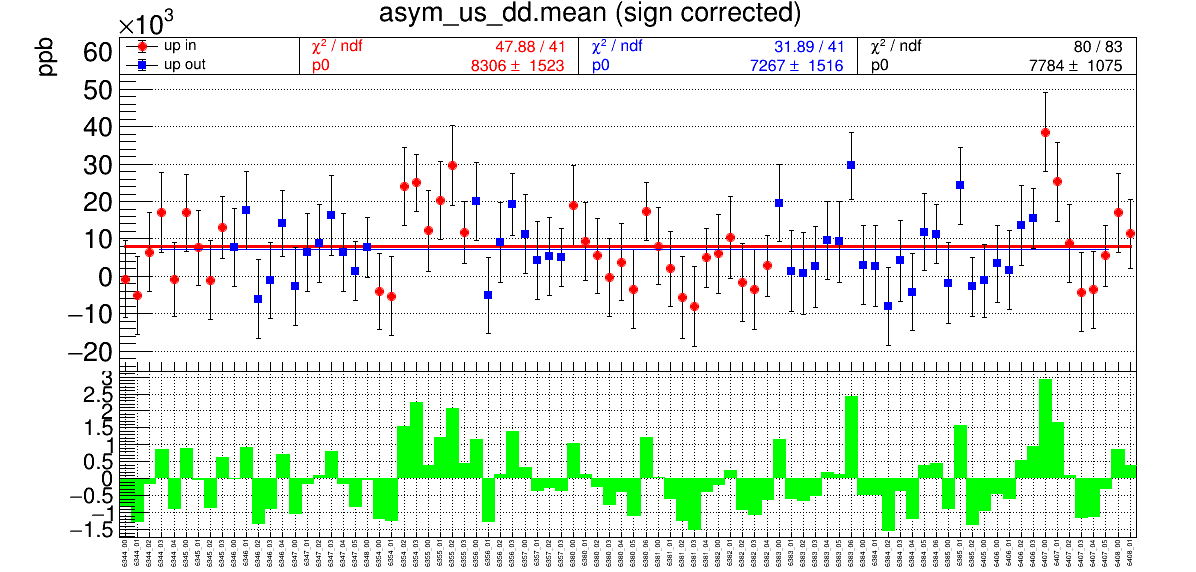
\includegraphics[width=0.9\linewidth]{at/mini_Ca48_asym_us_dd.mean.png}
    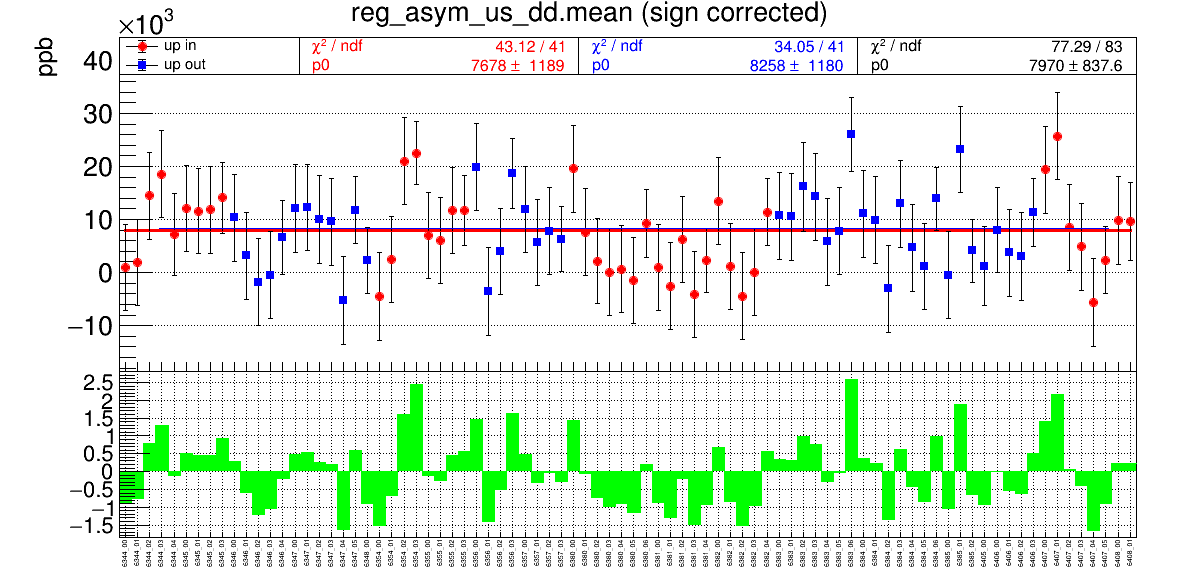
\includegraphics[width=0.9\linewidth]{at/mini_Ca48_reg_asym_us_dd.mean.png}
    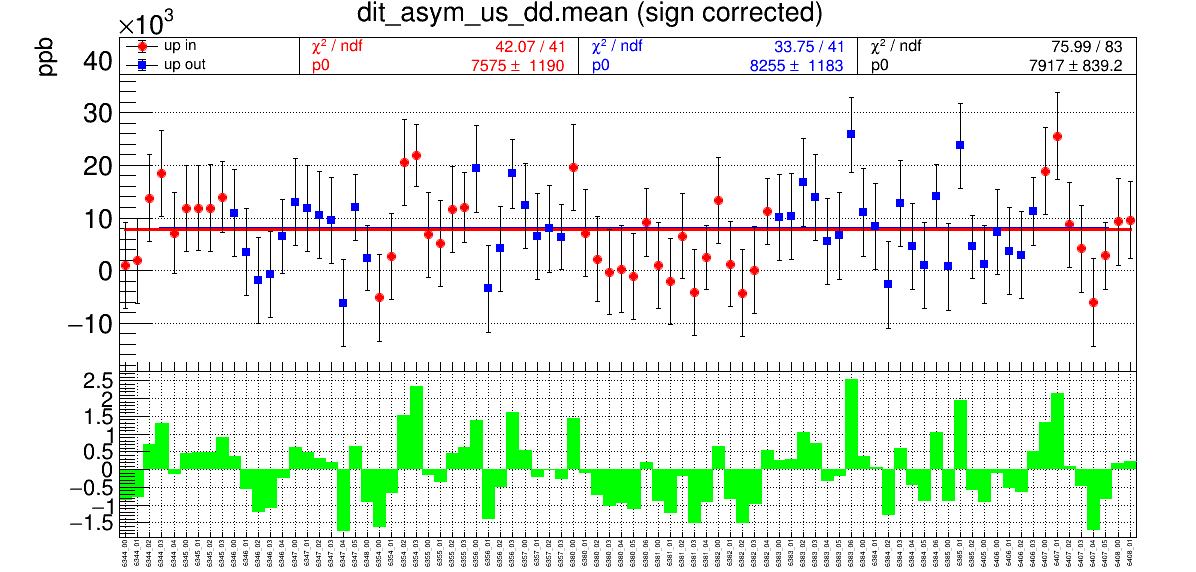
\includegraphics[width=0.9\linewidth]{at/mini_Ca48_dit_asym_us_dd.mean.png}
    \caption{Sign corrected minirun-average of raw, regression corrected and 
    dithering corrected transverse asymmetry of \Ca. Different colors represent
    different IHWP state (in/out). In each plot, the top pad shows the 
    mean and error of the title variable for each minirun, the 3 fit lines indicate
    fitting to IHWP=in, IHWP=out and all datapoints respectively;
    the bottom pad is the pull histogram, which is the ratio of the deviation 
    from the (all datapoints) mean value over each datapoint's error.
    % Regress with the following 5 BPMs: bpm1X, bpm4aY, bpm4eX, bpm4eY, bpm12X.
    % PREX-regression bpms: bpm4aX/Y, bpm4eX/Y, bpmE
    }
    \label{fig:AT_crex_Ca48_miniruns}
\end{figure}

\begin{figure}[H]
    \centering
    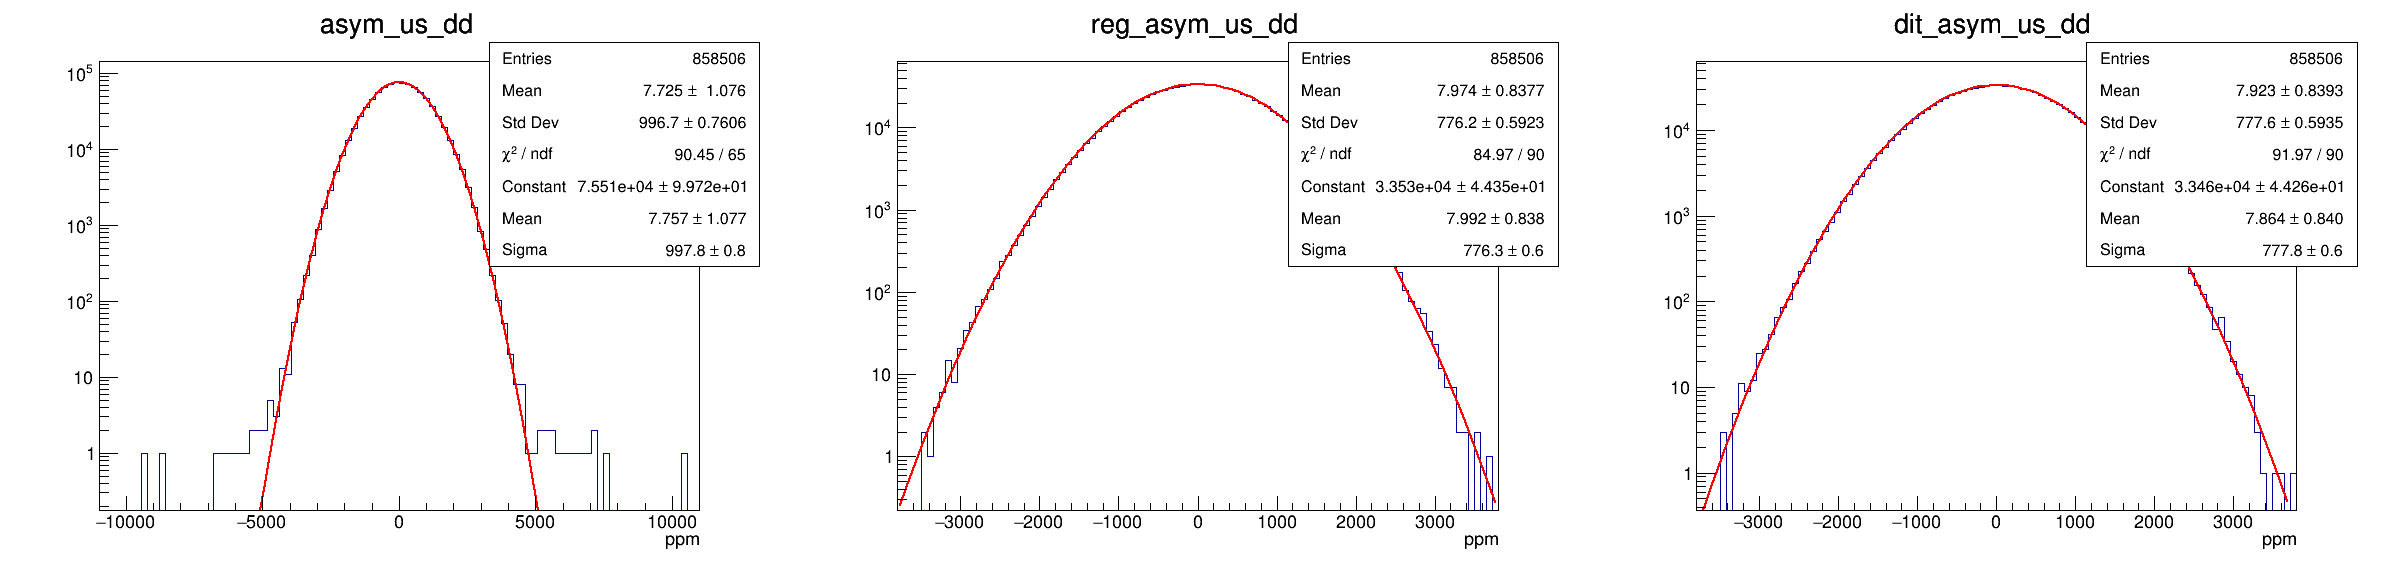
\includegraphics[width=\linewidth]{at/mulplot_Ca48}
    \caption{Mulplot for CREX \Ca. The red line is a Gaussian fit. One can see 
    clearly the how correction reduce the width of the distribution (note that
    the first plot has a larger x-range than the other two).}
    \label{fig:AT_crex_Ca48_mulplot}
\end{figure}

The minirun mean and mulplot mean for each target are summarized in the following
tables.
\begin{table}[!h]
    \scriptsize
    \begin{tabular}{c | r@{ $\pm$ }l r@{ $\pm$ }l r@{ $\pm$ }l | r@{ $\pm$ }l r@{ $\pm$ }l r@{ $\pm$ }l}
	\hline
	\multirow{2}{*}{Target}	& \multicolumn{6}{c|}{Minirun Average (ppb)} & \multicolumn{6}{c}{Mulplot (ppb)}	\\
	\cline{2-13}
	    & \multicolumn{2}{c}{raw}   & \multicolumn{2}{c}{reg}	& \multicolumn{2}{c|}{dit}   & \multicolumn{2}{c}{raw}	& \multicolumn{2}{c}{reg}   & \multicolumn{2}{c}{dit}	\\
	\hline
	\multicolumn{13}{c}{IHWP IN}   \\
	\hline
	\C	& 4205.3	& 1113.7    & 5173.9	& 501.5	    & 5169.4	& 502.1	    & 4129.8  & 1117.7    & 5105.0  & 504.9     & 5103.5  & 505.6   \\ 
	\ca	& 3055.9	& 1762.7    & 5507.5	& 419.3     & 5517.4	& 420.7	    & 2979.8  & 1763.3    & 5501.8  & 420.0     & 5511.7  & 421.4   \\   
	\Pb	& -266.2	& 974.2     & 54.9  	& 183.5     & 27.7  	& 185.7	    & -386.2  & 958.3     & 101.5   & 180.3     & 70.2    & 182.5   \\   
	\hline
	\multicolumn{13}{c}{IHWP OUT}   \\
	\hline
	\C	& 6111.0	& 992.1	    & 5685.5	& 437.4	    & 5740.6	& 437.9	    & 6055.9  & 995.8     & 5619.1  & 440.1     & 5669.4  & 440.6   \\ 
	\ca	& 5707.4	& 1687.6    & -679.8	& 443.0     & 5093.7	& 399.6	    & 5775.6  & 1687.8    & 5033.6  & 396.7     & 5033.6  & 399.2   \\   
	\Pb	& -132.7	& 927.4     & -52.3 	& 176.1     & -26.1 	& 178.7	    & -86.5   & 922.7     & -73.2   & 174.9     & -86.2   & 209.0   \\   
	\hline
	\multicolumn{13}{c}{COMBINED}   \\
	\hline
	\C	& 5267.8	& 740.8	    & 5464.5	& 329.6	    & 5493.9	& 330.0	    & 5209.7  & 743.5     & 5393.2  & 331.8     & 5427.0  & 332.2   \\ 
	\ca	& 4439.2	& 1219.0    & 5276.3	& 288.3     & 5294.7	& 289.7	    & 4444.9  & 1219.7    & 5275.3  & 288.5     & 5293.9  & 290.0   \\   
	\Pb	& -196.2	& 671.7     & -0.9  	& 127.0     & -0.3  	& 128.8	    & -231.5  & 664.7     & 11.3    & 125.5     & 70.2    & 182.5   \\   
	\hline
    \end{tabular}
    \caption{PREX-II raw and beam corrected transverse asymmetry}
\end{table}

\begin{table}[!h]
    \scriptsize
    \begin{tabular}{c | r@{ $\pm$ }l r@{ $\pm$ }l r@{ $\pm$ }l | r@{ $\pm$ }l r@{ $\pm$ }l r@{ $\pm$ }l}
	\hline
	\multirow{2}{*}{Target}	& \multicolumn{6}{c|}{Minirun Average (ppb)} & \multicolumn{6}{c}{Mulplot (ppb)}	\\
	\cline{2-13}
	    & \multicolumn{2}{c}{raw}   & \multicolumn{2}{c}{reg}	& \multicolumn{2}{c|}{dit}   & \multicolumn{2}{c}{raw}	& \multicolumn{2}{c}{reg}   & \multicolumn{2}{c}{dit}	\\
	\hline
	\multicolumn{13}{c}{IHWP IN}   \\
	\hline
	\C	& 6815.5    & 1397.2	& 7767.7    & 1182.2	& 7660.5    & 1183.4	& 6885.1    & 1397.9	& 7725.7    & 1182.1	& 7618.8 & 1183.3	\\ 
	\ca     & 8661.9    & 1643.5	& 8777.5    & 1265.2	& 8764.4    & 1267.5	& 8581.7    & 1645.3	& 8743.9    & 1265.3	& 8733.3 & 1267.6	\\ 
	\Ca     & 8306.5    & 1523.3   	& 7677.5    & 1188.9	& 7575.2    & 1190.3	& 8275.7    & 1524.9	& 7658.9    & 1189.0	& 7553.5 & 1190.3	\\ 
	\Pb	& 2742.6    & 2469.1   	& 3052.4    & 2285.9	& 3079.7    & 2288.1	& 2771.1    & 2469.6	& 3101.8    & 2286.2	& 3129.9 & 2288.3	\\ 
	\hline
	\multicolumn{13}{c}{IHWP OUT}   \\
	\hline
	\C	& 8607.9	& 1558.2    & 8789.1	& 1313.5    & 8791.5	& 1314.6    & 8512.9    & 1558.8	& 8778.2    & 1313.6	& 8780.0    & 1314.7	\\      
	\ca      & 8023.6	& 1751.5    & 7967.4	& 1353.3    & 7994.2	& 1355.0    & 8168.4    & 1755.1	& 7960.2    & 1353.4	& 7987.0    & 1355.2	\\      
	\Ca      & 7267.1	& 1516.3    & 8257.8	& 1180.2    & 8254.7	& 1183.3    & 7184.5    & 1517.6	& 8267.8    & 1180.3	& 8270.3    & 1183.5	\\      
	\Pb	& 2089.1	& 2456.4    & 2420.2	& 2263.4    & 2456.9	& 2266.2    & 2075.1    & 2456.8	& 2401.2    & 2263.8	& 2440.7    & 2266.6	\\      
	\hline
	\multicolumn{13}{c}{COMBINED}   \\
	\hline
	\C	& 7614.4	& 1040.3    & 8224.8	& 878.7     & 8166.8	& 879.5	    & 7600.8    & 1040.8	& 8235.1    & 878.8 	& 8177.3    & 879.6	\\      
	\Ca      & 8363.1	& 1198.5    & 8399.7	& 924.2     & 8405.0	& 925.6	    & 8377.3    & 1200.4	& 8383.5    & 924.3 	& 8390.4    & 925.7 	\\        
	\Ca  	& 7784.4	& 1074.7    & 7969.8	& 837.6     & 7916.9	& 839.2	    & 7725.4    & 1075.7	& 7974.4    & 837.7 	& 7923.5    & 839.3 	\\        
	\Pb      & 2414.2	& 1741.4    & 2733.1	& 1608.4    & 2765.3	& 1610.1    & 2422.6    & 1741.7	& 2751.0    & 1608.6	& 2784.8    & 1610.4	\\        
	\hline
    \end{tabular}
    \caption{PREX-II raw and beam corrected transverse asymmetry}
\end{table}

\begin{comment}
    & 343.4 & 154.8 & 155.1
    & 379.9 & 91.0  & 91.4
    & 493.9 & 93.0  & 94.1
    & 345.4 & 152.9 & 153.0
    & 387.2 & 91.3  & 91.9
    & 495.3 & 93.5  & 95.3
    & 344.5 & 153.7 & 153.9
    & 383.6 & 91.2  & 91.7
    & 494.5 & 93.2  & 94.6


\begin{table}
    \scriptsize
    \begin{tabular}{c | c c c | c c c}
	\hline
	\multirow{2}{*}{Target}	& \multicolumn{3}{c|}{Minirun Average (ppm)} & \multicolumn{3}{c}{Mulplot (ppm)}	\\
	\cline{2-7}
	    & raw	& reg	& dit	& raw	& reg	& dit	\\
	\hline
	\multicolumn{7}{c}{IHWP IN}   \\
	\hline
	C	& 659.82  & 558.10  & 558.71  & 659.84  & 557.97  & 558.56	\\
	Ca40    & 933.96  & 717.96  & 719.28  & 933.69  & 718.04  & 719.32	\\
	Ca48    & 994.35  & 775.30  & 776.19  & 994.78  & 775.61  & 776.50	\\
	Pb	& 1262.78 & 1168.89 & 1170.02 & 1261.95 & 1168.23 & 1169.35	\\
	\hline
	\multicolumn{7}{c}{IHWP OUT}   \\
	\hline
	C	& 8607.92 & 1558.19	& 8789.05 & 1313.51	& 8791.48 & 1314.60	 \\
	Ca40    & 8023.61 & 1751.48	& 7967.37 & 1353.29	& 7994.17 & 1355.00	 \\
	Ca48    & 7267.11 & 1516.31	& 8257.84 & 1180.23	& 8254.72 & 1183.33	 \\
	Pb	& 2089.10 & 2456.43	& 2420.15 & 2263.44	& 2456.87 & 2266.23	 \\
	\hline
	\multicolumn{7}{c}{COMBINED}   \\
	\hline
	C	& 661.92  & 558.72  & 559.27  & 661.73  & 558.75  & 559.29	\\
	Ca40    & 932.99  & 718.38  & 719.52  & 932.93  & 718.36  & 719.47	\\
	Ca48    & 996.46  & 775.93  & 777.46  & 996.67  & 776.15  & 777.63	\\
	Pb	& 1260.29 & 1163.94 & 1165.22 & 1259.54 & 1163.30 & 1164.57	\\
	\hline
    \end{tabular}
    \caption{Mini-wise average and mulplot average values for each target}
\end{table}
\end{comment}
As shown in above tables, the 2 correction methods -- regression and dithering 
match with each other,
We chose the dithering corrected values to extract transverse asymmetry.
A slug-wise plot of the transverse asymmetry are shown in Fig.~\ref{fig:AT_slug} 
\begin{figure}[H]
    \centering
    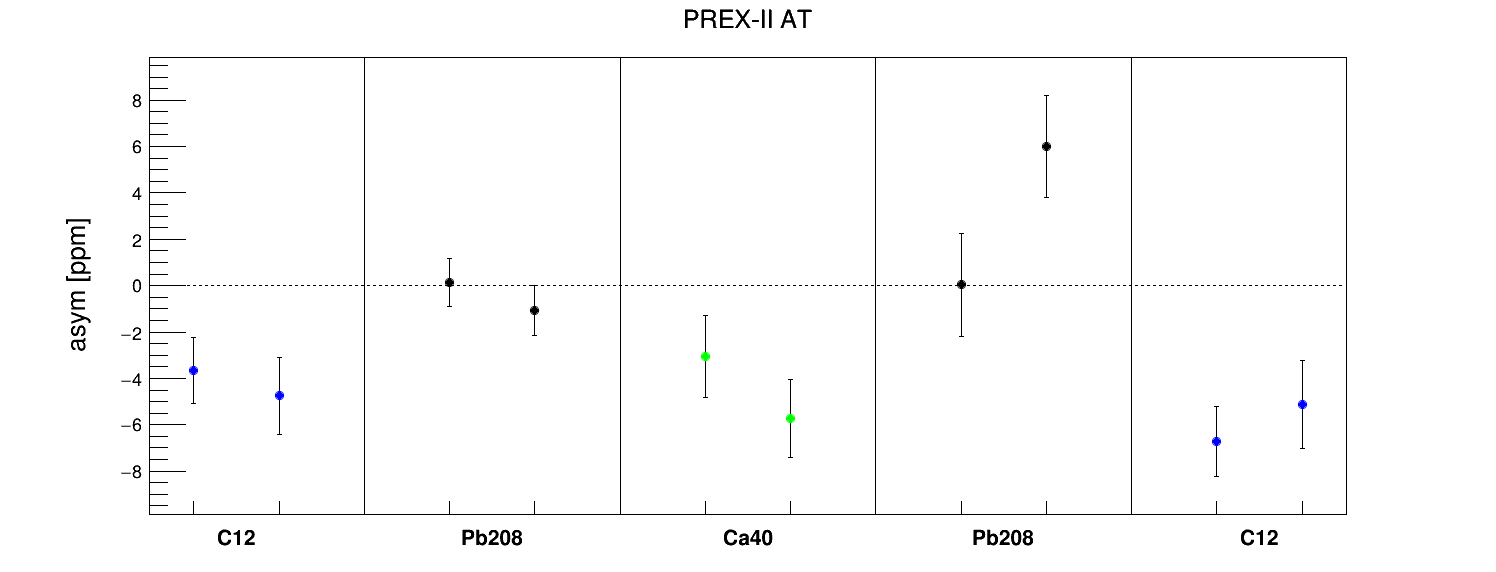
\includegraphics[width=\linewidth]{at/prex_at_slug}
    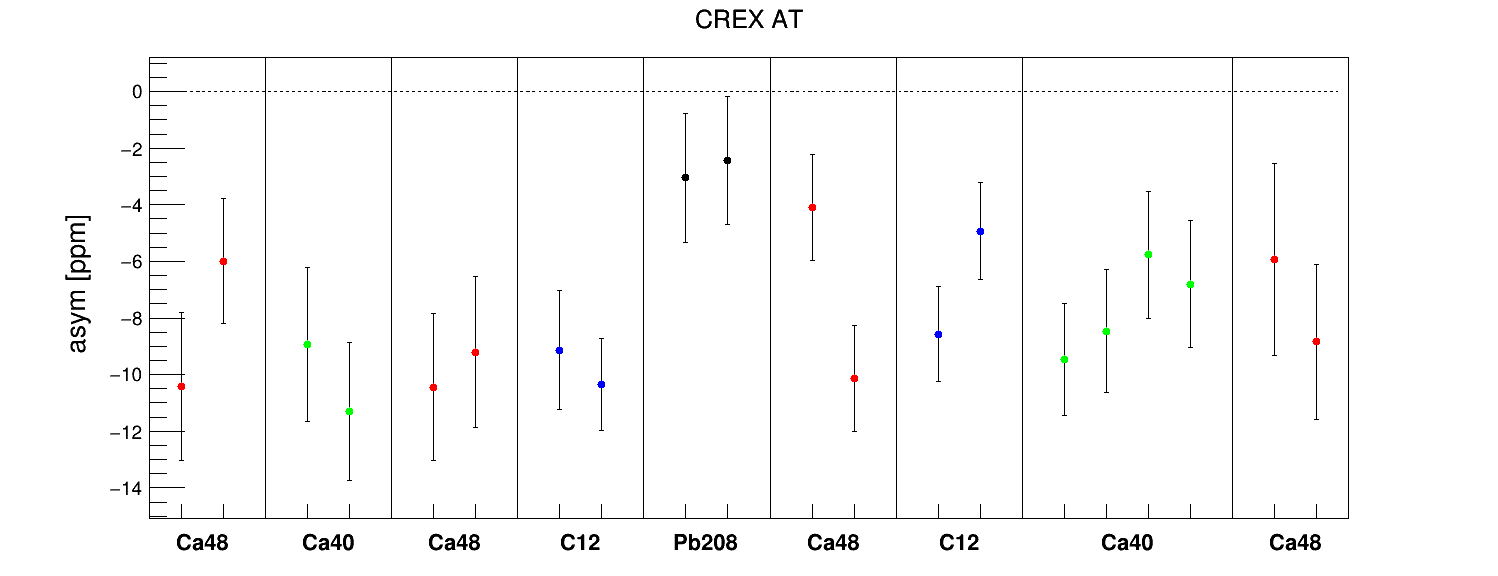
\includegraphics[width=\linewidth]{at/crex_at_slug}
    \caption{Sign corrected transverse asymmetry in chronological order. 
    Each datapoint means one slug.}
    \label{fig:AT_slug}
\end{figure}

%%%%%%%%%%%%%%%%%%%%%%%%%%%%%%%%%%%%%%%%%%%%%%%%
\subsection{Systematic Uncertainties}
Various corrections we made to the raw data will introduce corresponding uncertainties. 
Such as beam false asymmetry, purity correction and detector/monitor non-linearity correction. 
We need to know these correction precisely.

%%%%%%%%%%%%%%%%%%%%%%%%
\subsubsection{Beam Correction}
% https://prex.jlab.org/DocDB/0005/000504/002/Dithering%20and%20Regression.pdf
As said before, we used regression and dithering to extract detector's response
to beam fluctuations, and corrections from these 2 methods agreed with each other.
To count the uncertainty caused by beam correction, we used the difference 
between corrections of these 2 methods. More specifically, 
we found that for most runs, the difference between the corrections
of the most significant BPMs using these 2 methods was less than 5\%, therefore,
a conservative estimation of 5\% of the dithering correction was used as the 
beam correction systematic uncertainty. The dithering slope was target wise, 
the beam correction of each bpm (or their combinations) will be the product of 
the dithering slope and the average difference in each bpm (or their combinations), 
root-sum-square of 5\% of these corrections gave out the uncertainties. 
The result is shown below:

\begin{table}
    \centering
    \begin{tabular}{c c | c c | c c | c c | c}
	\hline
	Exp & Target	
	& \multicolumn{2}{c|}{\thead{$\CA_{raw} \pm d\CA_{raw}$ \\ (ppb)}}    
	& \multicolumn{2}{c|}{\thead{$\CA_{dit}  \pm d\CA_{dit}$ \\  (ppb)}}	
	& \multicolumn{2}{c|}{\thead{$\Delta\CA \pm d(\Delta\CA)$ \\ (ppb)}}	
	& $d\Delta\CA/d\CA_{dit}$\\
	\hline
	\multirow{3}{*}{PREX-II}
	    & \C    & -5268	& 741	& -5494	& 330	& 226.1	& 29.4	& 9\%	\\ 
	    & \ca   & -4439	& 1219	& -5295	& 290	& 195.9 & 42.4	& 15\%	\\ 
	    & \Pb   & 196.2	& 672	& 0.257	& 129	& 855.5 & 71.0	& 55\%	\\ 
	\hline
	\multirow{4}{*}{CREX}
	    & \C    & -7614	& 1040	& -8167	& 880	& 552.4 & 37.8	& 4\%	\\ 
	    & \ca   & -8363	& 1198	& -8405	& 926	& 351.1 & 48.9	& 5.3\%	\\ 
	    & \Ca   & -7784	& 1075	& -7917	& 839	& 41.9  & 86.7	& 10\%	\\ 
	    & \Pb   & -2414	& 1741	& -2765	& 1610	& 132.5 & 27.8	& 2\%	\\ 
	\hline
    \end{tabular}
    \caption{Beam correction to transverse asymmetry.}
\end{table}

%%%%%%%%%%%%%%%%%%%%%%%%
\subsubsection{Purity Correction}
For target purity correction, we need to consider only the \Pb and \Ca target.
As we will discuss in the following chapter, the contamination in the \Pb target
come from the diamond foils sandwiching the \Pb foil to cool the target, while
the impurity in \Ca target is mainly the \ca isotope. The \ca target has an abundance
larger than 99.6\%, so we regard it as a pure target.

\begin{equation}
    \begin{gathered}
	\CA_{mea} = \frac{R_t\CA_t + \sum_i R_i \CA_i}{R_t + \sum_i R_i} = \frac{\CA_t + \sum_i f_i \CA_i}{1 + \sum_i f_i}  \\
	\CA_t = (1 + \sum_i f_i)\CA_{mea} - \sum_i f_i\CA_i
    \end{gathered}
    \label{eq:AT-asymmetry_correction}
\end{equation}
where $R$ and $\CA$ are the scattering rate and asymmetry of each element, the
subscript t and i mean target and various impurity elements in the target, 
$f_i = \frac{R_i}{R_t}$ is the rate fraction. 
We used simulation to calculate the scattering rate for each different
target, asymmetry value was what we measured.

\begin{equation}
    f_C = \frac{R_C}{R_{Pb}} = 
    \begin{cases}
	0.0671 \pm 0.0057   & E = 0.95\ GeV	\\
	0.6089 \pm 0.0609   & E = 2.2\ GeV	\\
    \end{cases}
\end{equation}

The \Ca case was a little complicated, because the \Ca target was a stack of 3 different
pieces with different purity. The upstream 2 pieces were the remnant of the destroyed
old target with a \Ca abundance of 95.99\%, the downstream piece was a new foil
with a \Ca abundance of 90.04\%. Based on the fact that contamination was isotope
of \Ca: \ca ($\sim10\%$), ${}^{42}Ca$ ($\sim0.1\%$) and ${}^{44}Ca$ ($\sim0.2\%$), whose 
scattering rate and asymmetry are similar to that of \Ca, so we calculated the
non-\Ca fraction in the \Ca target, which gave the rate fraction as: 
$f(\frac{non-{}^{48}Ca}{{}^{48}Ca}) = 9.07 \pm 0.18 \%$.

Using equation \ref{eq:AT-asymmetry_correction}, we get the purity corrected
asymmetries:
\begin{table}
% https://docs.google.com/spreadsheets/d/1ZI68PgAn_zySKozZ__kHBvxlBmaTMKw9jPSl-EIa91k/edit?pli=1#gid=1243115322
% why cell J4 doesn't follow error propagation
% K3-K9: the formula looks weird
    \centering
    \begin{tabular}{c c | c c }
	\hline
	Exp & Target	
	& \multicolumn{2}{c}{$\CA_{cor}  \pm d\CA_{stat}$ (ppb)}	    \\
	\hline
	\multirow{3}{*}{PREX-II}
	    & \C    & -5494	& 330	 \\ 
	    & \Ca   & -5295	& 290	 \\ 
	    & \Pb   & 369	& 137	 \\ 
	\hline
	\multirow{4}{*}{CREX}
	    & \C    & -8167	& 880	 \\ 
	    & \ca   & -8405	& 926	 \\ 
	    & \Ca   & -7873	& 919	 \\ 
	    & \Pb   & 523	& 2646	 \\ 
	\hline
    \end{tabular}
    \caption{Purity corrected transverse asymmetry. The statistical uncertainties
    were calculated following uncertainty propagation equation.}
\end{table}

%%%%%%%%%%%%%%%%%%%%%%%%
\subsubsection{Detector Non-linearity}
For uncertainty caused by detector non-linearity response to the incoming electron flux,
it was bounded to be $<0.5\%$ in bench tests.
\begin{table}[!h]
    \centering
    \begin{tabular}{c c | c c c}
	\hline
	Exp & Target	& $\CA_{raw}$ (ppb) & $d\CA_{sys}$ (ppb)    & $\frac{d\CA_{sys}}{\CA_{raw}}$   \\
	\hline
	\multirow{3}{*}{PREX-II}
	    & \C    & -5268	& 26	& 0.50\%    \\ 
	    & \ca   & -4439	& 22	& 0.50\%    \\ 
	    & \Pb   & 196.2	& 1	& 0.50\%    \\ 
	\hline
	\multirow{4}{*}{CREX}
	    & \C    & -7614	& 38	& 0.50\%    \\ 
	    & \ca   & -8363	& 42	& 0.50\%    \\ 
	    & \Ca   & -7784	& 39	& 0.50\%    \\ 
	    & \Pb   & -2414	& 12	& 0.50\%    \\ 
	\hline
    \end{tabular}
    \caption{Systematic uncertainty due to detector non-linearity}
\end{table}

For uncertainty come from bcm non-linearity, a conservative estimation of 1\% was used,
as shown in Table~\ref{tab:AT_bcm_non-linearity}, the charge asymmetry was minirun-wise average 
value.
\begin{table}[!h]
    \centering
    \begin{tabular}{c c | c c c}
	\hline
	Exp & Target	& $\CA_{q}$ (ppb) & $d\CA_{q}$ (ppb)    & $\frac{d\CA_{q}}{\CA_{q}}$   \\
	\hline
	\multirow{3}{*}{PREX-II}
	    & \C    & -52.863   & 0.5   & 1.00\%    \\ 
	    & \ca   & -104.763  & 1.0   & 1.00\%    \\ 
	    & \Pb   & 140.602   & 1.4   & 1.00\%    \\ 
	\hline
	\multirow{4}{*}{CREX}
	    & \C    & 50.09	& 0.5   & 1.00\%    \\ 
	    & \ca   & 47.81	& 0.5   & 1.00\%    \\ 
	    & \Ca   & 27.35	& 0.3   & 1.00\%    \\ 
	    & \Pb   & -1.61	& 0.0   & 1.00\%    \\ 
	\hline
    \end{tabular}
    \caption{Systematic uncertainty due to BCM non-linearity}
    \label{tab:AT_bcm_non-linearity}
\end{table}

%%%%%%%%%%%%%%%%%%%%%%%%%%%%%%%%%%%%%%%%%%%%%%%%
\subsection{Dynamics}

%%%%%%%%%%%%%%%%%%%%%%%%
\subsubsection{$\phi$ Angle}
% http://ace.phys.virginia.edu/HAPPEX/4179
% http://ace.phys.virginia.edu/HAPPEX/4179
We said above that we chose the angle $\phi$ to be $90^\circ$, but no way to 
achieve exactly that value. The actually value will be a little deviate from
the designed value, as we measured from the data. We draw the $\sin\phi$ distribution
from data, and then took the average, as shown in the following table:
\begin{table}[!htbp]
    \centering
    \begin{tabular}{c c | c c c}
	\hline
	Exp & Target	& LHRS $\sin\phi$   & RHRS $\sin\phi$	& average   \\
	\hline
	\multirow{3}{*}{PREX-II}
	    & \C    & 0.96660   & 0.96700	& 0.9668    \\ 
	    & \ca   & 0.96430   & 0.96440	& 0.9644    \\ 
	    & \Pb   & 0.96625   & 0.96665	& 0.9665    \\ 
	\hline
	\multirow{4}{*}{CREX}
	    & \C    & 0.96950   & 0.96790	& 0.9687    \\ 
	    & \ca   & 0.97090   & 0.96920	& 0.9701    \\ 
	    & \Ca   & 0.97110   & 0.96880	& 0.9700    \\ 
	    & \Pb   & 0.96980   & 0.96830	& 0.9691    \\ 
	\hline
    \end{tabular}
    \caption{Average $\sin\phi$ values for different AT targets.}
\end{table}

%%%%%%%%%%%%%%%%%%%%%%%%
\subsubsection{$Q^2$}
Similar to the extraction of $\phi$ angle, we draw the $Q^2$ distribution for
each target, and then took the mean value. The results are shown in the
following table:
% http://ace.phys.virginia.edu/HAPPEX/4453
% http://ace.phys.virginia.edu/HAPPEX/4468
\begin{table}[!htbp]
    \centering
    \begin{tabular}{c c | r@{ $\pm$ }l | r@{ $\pm$ }l | r@{ $\pm$ }l r@{ $\pm$ }l}
	\hline
	Exp & Target	
	& \multicolumn{2}{c|}{\thead{LHRS $Q^2$ \\ ($GeV^2$)}} 
	& \multicolumn{2}{c|}{\thead{RHRS $Q^2$ \\ ($GeV^2$)}} 
	& \multicolumn{2}{c}{\thead{Average $Q^2$ \\ ($GeV^2$)}} & \multicolumn{2}{c}{\thead{Average $Q$ \\ ($GeV$)}} \\
	\hline
	\multirow{4}{*}{PREX-II}
	& \C	& 0.0068    & 4E-6  & 0.0066    & 5E-6	& 0.00671   & 3.21E-6	& 0.082	& 1.96E-5	\\
	& \ca  	& 0.0068    & 5E-6  & 0.0067    & 6E-6  & 0.00673   & 4.17E-6  & 0.082	& 2.54E-5	\\
	& \Pb 8	& 0.0065    & 5E-6  & 0.0063    & 6E-6  & 0.00640   & 4.06E-6  & 0.080	& 2.54E-5	\\
	& \Pb 9	& 0.0065    & 4E-6  & 0.0063    & 5E-6  & 0.00640   & 3.50E-6  & 0.080	& 2.18E-5	\\
	\hline
	\multirow{4}{*}{CREX}
	& \C	& 0.0328    & 2E-5  & 0.0334    & 2E-5	& 0.0331    & 1.31E-5  & 0.182	& 3.61E-5	\\
	& \ca  	& 0.0306    & 2E-5  & 0.0309    & 2E-5	& 0.0308    & 1.22E-5  & 0.175	& 3.48E-5	\\
	& \Ca  	& 0.0304    & 1E-5  & 0.0307    & 2E-5	& 0.0306    & 1.07E-5  & 0.175	& 3.05E-5	\\
	& \Pb	& 0.0319    & 3E-5  & 0.0322    & 3E-5	& 0.0320    & 1.99E-5  & 0.179	& 5.56E-5	\\
	\hline
    \end{tabular}
    \caption{Average $Q^2$ values for different AT targets.}
\end{table}

%%%%%%%%%%%%%%%%%%%%%%%%%%%%%%%%%%%%%%%%%%%%%%%%
\subsection{Final Result}
From Eq.~\ref{eq:measured_AT}, we can calculate the transverse asymmetry:
\begin{equation}
    \CA_n = \frac{\CA_{cor}}{P_n \cdot \sin\phi}
\end{equation}

The statistical uncertainty was calculated as:
\begin{equation}
    d\CA_n(stat) = \frac{d\CA_{cor}(stat)}{P_n \cdot \sin\phi}
\end{equation}

The systematic uncertainty was calculated as:
\begin{equation}
    \left( \frac{d\CA_n(sys)}{\CA_n} \right)^2 = 
	\left( \frac{d\CA_{cor}(sys)}{d\CA_{cor}} \right)^2
	+ \left( \frac{dP_n}{P_n}\right)^2 
\end{equation}
where
\begin{equation}
    d\CA^2_{cor}(sys) = d\CA^2(det\ nonlin) + d\CA^2(bcm\ nonlin) + d\CA^2(beam\ correction)
\end{equation}
In case of \Pb and \Ca target, we need to include uncertainties from contaminations.
Various systematic uncertainties are summarized in Table~\ref{tab:AT_uncertainties}.
\begin{table}[!h]
    \centering
    \begin{tabular}{c c c c | c c c c}
	\hline
	Exp & \multicolumn{3}{c|}{PREX-II}  & \multicolumn{4}{c}{CREX}	\\
	Target	& \C	& \ca	& \Pb	& \C	& \ca	& \Ca	& \Pb	\\
	\hline
	Beam correction & 0.03  & 0.05  & 0.08  & 0.04  & 0.06  & 0.10  & 0.03	\\
	Polarization    & 0.06  & 0.05  & $<0.01$ & 0.08  & 0.08  & 0.08  & $<0.01$	\\
	Non-linearity   & 0.03  & 0.03  & $<0.01$ & 0.05  & 0.05  & 0.05  & 0.01	\\
	Tgt. impurity   & $<0.01$ & $<0.01$ & 0.04  & $<0.01$ & $<0.01$ & 0.10  & 0.80	\\
	Inelastic	& $<0.01$ & $<0.01$ & $<0.01$ & 0.08  & 0.15  & 0.08  & $<0.01$	\\
	\hline	
	Tot. Syst	& 0.07  & 0.08  & 0.09  & 0.13  & 0.18  & 0.19  & 0.75	\\
	Statistical	& 0.38  & 0.34  & 0.16  & 1.05  & 1.10  & 1.09  & 3.15	\\
	Total		& 0.39  & 0.34  & 0.18  & 1.05  & 1.11  & 1.11  & 3.23	\\
	\hline
    \end{tabular}
    \caption{AT uncertainty contributions in unit of ppm}
    \label{tab:AT_uncertainties}
\end{table}

The final result is shown in Table~\ref{tab:AT_final_values}:
\begin{table}[!h]
    \centering
    \begin{tabular}{c c | c c c c}
	\hline
	Exp & Target	& \thead{$\CA_n$ \\ (ppm)}   & \thead{$d\CA_{stat}$ \\ (ppm)}	
	& \thead{$d\CA_{sys}$ \\ (ppm)}	& \thead{$d\CA_{stat+sys}$ \\ (ppm)}	\\
	\hline
	\multirow{3}{*}{PREX-II}
	    & \C    & -6.34	& 0.38	& 0.07	& 0.39	\\ 
	    & \ca   & -6.12	& 0.34	& 0.08	& 0.34	\\ 
	    & \Pb   & 0.43	& 0.16	& 0.09	& 0.18	\\ 
	\hline
	\multirow{4}{*}{CREX}
	    & \C    & -9.71	& 1.05	& 0.10	& 1.05	\\ 
	    & \ca   & -9.98	& 1.10	& 0.11	& 1.11	\\ 
	    & \Ca   & -9.35	& 1.09	& 0.17	& 1.11	\\ 
	    & \Pb   & 0.62	& 3.15	& 0.75	& 3.23	\\ 
	\hline
    \end{tabular}
    \caption{Final result of Transverse asymmetry.}
    \label{tab:AT_final_values}
\end{table}

Compare to theoretical calculation \cite{PhysRevC.103.064316}, we confirm 
the anomaly appeared in PREX-I, that is the \Pb transverse asymmetries
are consistently 0 at various $Q$ values, as shown in Fig.~\ref{fig:pcrex_AT}. 
As for other light nuclei, they are not far away from theoretical predictions.
\begin{figure}
    \centering
    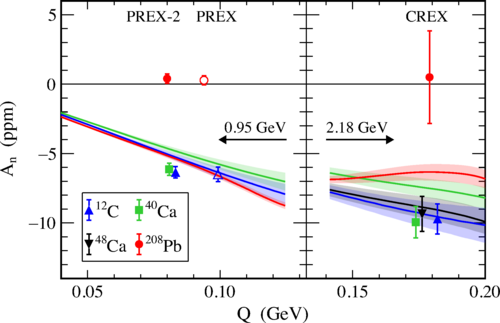
\includegraphics[scale=.5]{at/pcrex_AT}
    \caption{Transverse asymmetry measured in PREX-II/CREX. The PREX-I result
    is also included. Overlapping points are offset slightly in Q to distinguish
    them.}
    \label{fig:pcrex_AT}
\end{figure}

\begin{comment}
    \begin{itemize}
	\item resource: AT plot: https://github.com/cipriangal/prexATplot
	\item regression: which bpm set were used?
	\item dithering: ???
	\item 
    \end{itemize}
\end{comment}
